% Copyright 2004 by Till Tantau <tantau@users.sourceforge.net>.
%
% In principle, this file can be redistributed and/or modified under
% the terms of the GNU Public License, version 2.
%
% However, this file is supposed to be a template to be modified
% for your own needs. For this reason, if you use this file as a
% template and not specifically distribute it as part of a another
% package/program, I grant the extra permission to freely copy and
% modify this file as you see fit and even to delete this copyright
% notice. 

\documentclass{beamer}

% There are many different themes available for Beamer. A comprehensive
% list with examples is given here:
% http://deic.uab.es/~iblanes/beamer_gallery/index_by_theme.html
% You can uncomment the themes below if you would like to use a different
% one:
\usetheme{AnnArbor}
%\usetheme{Antibes}
%\usetheme{Bergen}
%\usetheme{Berkeley}
%\usetheme{Berlin}
%\usetheme{Boadilla}
%\usetheme{boxes}
%\usetheme{CambridgeUS}
%\usetheme{Copenhagen}
%\usetheme{Darmstadt}
%\usetheme{default}
%\usetheme{Frankfurt}
%\usetheme{Goettingen}
%\usetheme{Hannover}
%\usetheme{Ilmenau}
%\usetheme{JuanLesPins}
%\usetheme{Luebeck}
%\usetheme{Madrid}
%\usetheme{Malmoe}
%\usetheme{Marburg}
%\usetheme{Montpellier}
%\usetheme{PaloAlto}
%\usetheme{Pittsburgh}
%\usetheme{Rochester}
%\usetheme{Singapore}
%\usetheme{Szeged}
%\usetheme{Warsaw}

\definecolor{uofsgreen}{rgb}{.125,.5,.25}
\usecolortheme{beaver}
%\usecolortheme[named=uofsgreen]{structure}
%\setbeamercolor{titlelike}{bg=white}
%\setbeamercolor{frametitle}{fg=uofsgreen,bg=white}

% changing the color to uofsgreen
\definecolor{darkred}{rgb}{.125,.5,.25}

\setbeamercolor{section in toc}{fg=black,bg=white}
\setbeamertemplate{section in toc}{%
  {\color{uofsgreen!70!black}\inserttocsectionnumber.}~\inserttocsection}
\setbeamertemplate{subsection in toc}{%
  \hspace{1.2em}{\color{uofsgreen}\rule[0.3ex]{3pt}{3pt}}~\inserttocsubsection\par}
  
%\setbeamercolor{section in toc shaded}{fg=uofsgreen,bg=white}
\setbeamercolor{alerted text}{fg=darkred!80!gray}
\setbeamercolor*{palette primary}{fg=darkred!60!black,bg=gray!30!white}
\setbeamercolor*{palette secondary}{fg=darkred!70!black,bg=gray!15!white}
\setbeamercolor*{palette tertiary}{bg=darkred!80!black,fg=gray!10!white}
\setbeamercolor*{palette quaternary}{fg=darkred,bg=gray!5!white}

\setbeamercolor*{sidebar}{fg=darkred,bg=gray!15!white}

\setbeamercolor*{palette sidebar primary}{fg=darkred!10!black}
\setbeamercolor*{palette sidebar secondary}{fg=white}
\setbeamercolor*{palette sidebar tertiary}{fg=darkred!50!black}
\setbeamercolor*{palette sidebar quaternary}{fg=gray!10!white}

%\setbeamercolor*{titlelike}{parent=palette primary}
\setbeamercolor{titlelike}{parent=palette primary,fg=darkred}
\setbeamercolor{title}{parent=palette primary,fg=darkred}
\setbeamercolor{frametitle}{bg=gray!10!white}
\setbeamercolor{frametitle right}{bg=gray!60!white}
\setbeamercolor{normal text}{parent=palette quaternary}
\setbeamercolor{itemized item}{parent=palette tertiary}

\setbeamercolor*{separation line}{}
\setbeamercolor*{fine separation line}{}

\newenvironment{bulletenv}{\only{\setbeamercolor{local structure}{fg=uofsgreen}}}{}

\title{Borealis Project Update}

% A subtitle is optional and this may be deleted
\subtitle{A Digital Radar Design for SuperDARN Using Software-Defined Radios}

\author{K.~Kotyk \and K.~Krieger \and M.~Detwiller \and K.~McWilliams \and J-P.~St.~Maurice}
% - Give the names in the same order as the appear in the paper.
% - Use the \inst{?} command only if the authors have different
%   affiliation.

\institute[University of Saskatchewan] % (optional, but mostly needed)
% {
%   \inst{1}%
%   University of Saskatchewan
%   \and
%   \inst{2}
%   University of Saskatchewan}
% - Use the \inst command only if there are several affiliations.
% - Keep it simple, no one is interested in your street address.

\date{SuperDARN Workshop, 2018}
% - Either use conference name or its abbreviation.
% - Not really informative to the audience, more for people (including
%   yourself) who are reading the slides online

\subject{Borealis Project Update}
% This is only inserted into the PDF information catalog. Can be left
% out. 

% If you have a file called "university-logo-filename.xxx", where xxx
% is a graphic format that can be processed by latex or pdflatex,
% resp., then you can add a logo as follows:

\pgfdeclareimage[height=0.5cm]{university-logo}{usask-usask-colour.eps} % MD: never use underscores in file names when using latex, use gimp to export to eps
\logo{\pgfuseimage{university-logo}}

% Delete this, if you do not want the table of contents to pop up at
% the beginning of each subsection:
% \AtBeginSubsection[]
% {
%   \begin{frame}<beamer>{Outline}
%     \tableofcontents[currentsection,currentsubsection]
%   \end{frame}
% }

% Let's get started
\begin{document}

\begin{frame}
  \titlepage
\end{frame}

\begin{frame}{Outline}
  \tableofcontents
  % You might wish to add the option [pausesections]
\end{frame}

% Section and subsections will appear in the presentation overview
% and table of contents.
\section{Project Motivation}

\subsection{Deprecated Systems}

\begin{frame}
% \frametitle{Project Motivation}
  \begin{columns}[T]
    \begin{column}{.5\textwidth}
      \begin{block}{}
     \begin{itemize}
      \item<bullet@1-> Deprecated GC214 Receiver Card
      \item<bullet@1-> QNX4
     \end{itemize}
% Your text here
    \end{block}
    \end{column}
    
    \begin{column}{.5\textwidth}
    \begin{block}{}
% Your image included here
    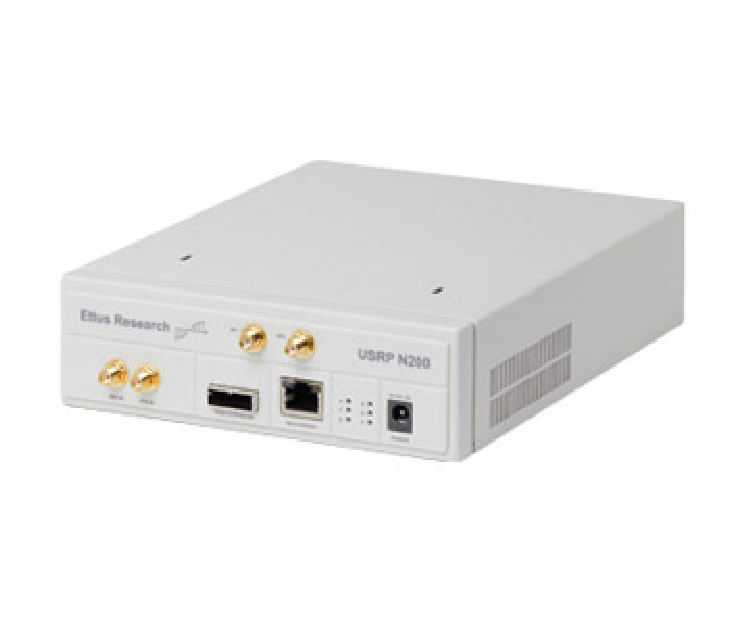
\includegraphics[width=\textwidth]{n200.eps}
    \end{block}
    \end{column}
  \end{columns}
\end{frame}

\subsection{Increase Capabilities}

\section{Hardware}

\subsection{Ettus Universal Software Radio Peripherals (USRPs)}

\begin{frame}
\frametitle{Ettus Universal Software Radio Peripheral}
  \begin{columns}[T]
    \begin{column}{.5\textwidth}
     \begin{block}{Your textblock}
% Your text here
    \end{block}
    \end{column}
    \begin{column}{.5\textwidth}
    \begin{block}{}
% Your image included here
    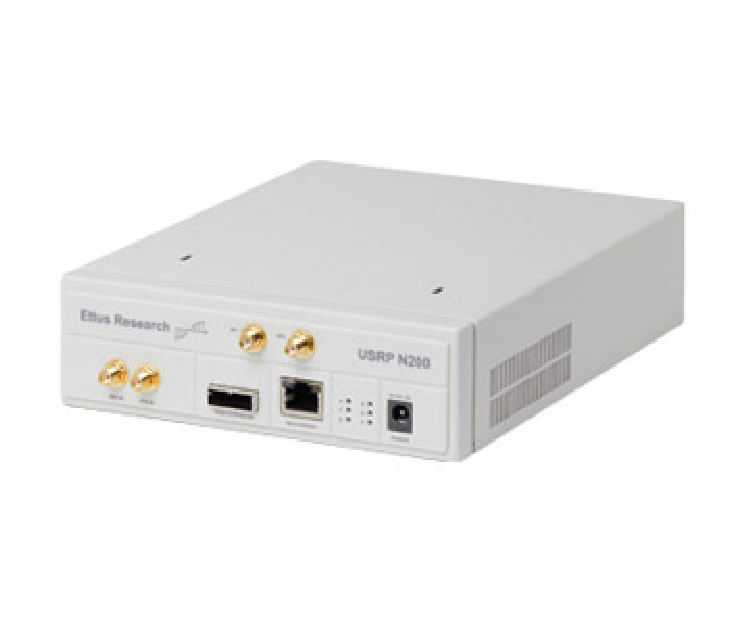
\includegraphics[width=\textwidth]{n200.eps}
    \end{block}
    \end{column}
  \end{columns}
\end{frame}

\begin{frame}
\frametitle{Ettus Universal Software Radio Peripheral}
  \begin{columns}[T]
    \begin{column}{.5\textwidth}
     \begin{block}{Your textblock}
% Your text here
    \end{block}
    \end{column}
    \begin{column}{.5\textwidth}
    \begin{block}{}
% Your image included here
    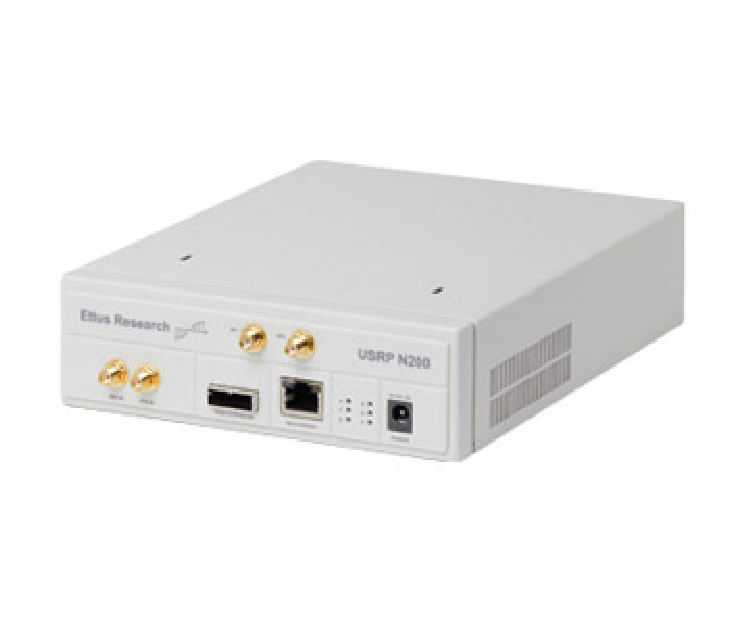
\includegraphics[width=\textwidth]{n200.eps}
    \end{block}
    \end{column}
  \end{columns}
\end{frame}

\section{Software}

\subsection{Design Goals}

\subsection{Creating Experiments}

\subsection{Features}

\section{Progress}

\subsection{Current Status}

\subsection{Issues}

\subsection{Next Steps}

\subsection{First Results}

\begin{frame}
\frametitle{Ettus Universal Software Radio Peripheral}
  \begin{columns}[T]
    \begin{column}{.5\textwidth}
     \begin{block}{Your textblock}
% Your text here
    \end{block}
    \end{column}
    \begin{column}{.5\textwidth}
    \begin{block}{}
% Your image included here
    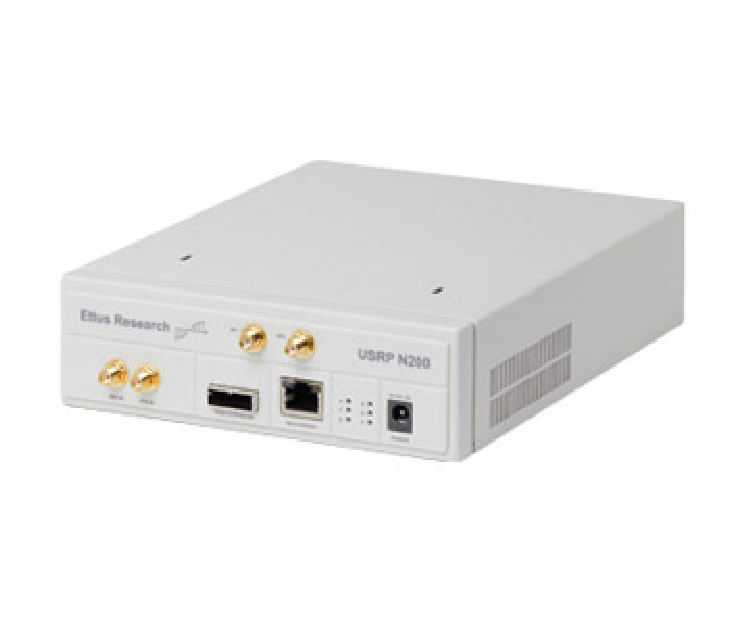
\includegraphics[width=\textwidth]{n200.eps}
    \end{block}
    \end{column}
  \end{columns}
\end{frame}

% You can reveal the parts of a slide one at a time
% with the \pause command:
% \begin{frame}{Second Slide Title}
%   \begin{itemize}
%   \item {
%     First item.
%     \pause % The slide will pause after showing the first item
%   }
%   \item {   
%     Second item.
%   }
%   % You can also specify when the content should appear
%   % by using <n->:
%   \item<3-> {
%     Third item.
%   }
%   \item<4-> {
%     Fourth item.
%   }
%   % or you can use the \uncover command to reveal general
%   % content (not just \items):
%   \item<5-> {
%     Fifth item. \uncover<6->{Extra text in the fifth item.}
%   }
%   \end{itemize}
% \end{frame}
%
% \section{Second Main Section}
%
% \subsection{Another Subsection}
%
% \begin{frame}{Blocks}
% \begin{block}{Block Title}
% You can also highlight sections of your presentation in a block, with it's own title
% \end{block}
% \begin{theorem}
% There are separate environments for theorems, examples, definitions and proofs.
% \end{theorem}
% \begin{example}
% Here is an example of an example block.
% \end{example}
% \end{frame}
%
% % Placing a * after \section means it will not show in the
% % outline or table of contents.
% \section*{Summary}
%
% \begin{frame}{Summary}
%   \begin{itemize}
%   \item
%     The \alert{first main message} of your talk in one or two lines.
%   \item
%     The \alert{second main message} of your talk in one or two lines.
%   \item
%     Perhaps a \alert{third message}, but not more than that.
%   \end{itemize}
%   
%   \begin{itemize}
%   \item
%     Outlook
%     \begin{itemize}
%     \item
%       Something you haven't solved.
%     \item
%       Something else you haven't solved.
%     \end{itemize}
%   \end{itemize}
% \end{frame}
%
%
%
% % All of the following is optional and typically not needed. 
% \appendix
% \section<presentation>*{\appendixname}
% \subsection<presentation>*{For Further Reading}
%
% \begin{frame}[allowframebreaks]
%   \frametitle<presentation>{For Further Reading}
%     
%   \begin{thebibliography}{10}
%     
%   \beamertemplatebookbibitems
%   % Start with overview books.
%
%   \bibitem{Author1990}
%     A.~Author.
%     \newblock {\em Handbook of Everything}.
%     \newblock Some Press, 1990.
%  
%     
%   \beamertemplatearticlebibitems
%   % Followed by interesting articles. Keep the list short. 
%
%   \bibitem{Someone2000}
%     S.~Someone.
%     \newblock On this and that.
%     \newblock {\em Journal of This and That}, 2(1):50--100,
%     2000.
%   \end{thebibliography}
% \end{frame}

\end{document}
